\documentclass[11pt]{article}
\usepackage[a4paper,margin=25mm]{geometry}
\usepackage[T1]{fontenc}
\usepackage[utf8]{inputenc}
\usepackage{lmodern}
\usepackage{graphicx}
\usepackage{booktabs}
\usepackage{amsmath}
\usepackage{xspace}
\usepackage{hyperref}
\graphicspath{{../fullsim_analysis/results/2026-10_ambient/room_temperature/}}
\newcommand{\us}{\textmu s\xspace}
\newcommand{\Na}{\ensuremath{{}^{22}\mathrm{Na}}\xspace}
\newcommand{\Vov}{\ensuremath{V_{\rm ov}}\xspace}
\newcommand{\csitl}{CsI(Tl)\xspace}

\title{BGO and \csitl crystals read by 64 SiPMs at room temperature:\\
a simulation of three readouts}
\author{J.\,J.~Gómez-Cadenas}
\date{19 October 2026}

\begin{document}
\maketitle

\begin{abstract}
We simulate the response of two $48 \times 48$~mm$^2$ scintillating
crystals, BGO and \csitl, read through optical grease by an $8 \times 8$
array of SiPMs at room temperature and irradiated by a \Na source. The
simulation follows each decay from the gamma interactions in the crystal to
the charge recorded by three readouts: the Citiroc~1A and the Radioroc2,
two ASICs that shape the signal and store its maximum, and the CAEN DT2745,
a waveform digitiser whose records are integrated offline. For each of the
six combinations of crystal and readout we determine the trigger, the
calibration of the SiPM gain from their dark counts, the energy spectrum,
the energy resolution at 511~keV and the number of photoelectrons. The
crystals produce 3885 (BGO) and 27\,600 (\csitl) photons per 511~keV
deposit, of which 84\% reach the SiPMs and 49 to 50\% (BGO) or 31 to 41\%
(\csitl) become photoelectrons. On samples of 10\,000 decays the energy
resolution is 11.1, 9.2 and 9.2\% FWHM for BGO and 8.3, 6.2 and 6.0\% for
\csitl with the Citiroc, the digitiser and the Radioroc2 respectively,
with an uncertainty of 0.2 points. The intrinsic resolution of the
crystals, taken as 5\%, and the statistics of the photoelectrons account
for most of the width; the readout adds a contribution that is largest for
the Citiroc, whose voltage-sensitive preamplifiers and short shaping keep
about a third of the BGO light and an eighth of the \csitl light. The dark
counts of the SiPMs at room temperature, about 4~MHz per channel, set the
trigger thresholds and allow the calibration of the two ASICs only at a
short shaping of their high-gain path, 25~ns for the Citiroc and 100~ns for
the Radioroc2, the energy being read on the low-gain path. The pulse of the
SiPM, computed from its capacitance and the input resistance of the
readout, and the electronic noise of the ASICs are estimates, and the
operating conditions are proposals of the simulation, to be confirmed by
the first measurements.
\end{abstract}

\tableofcontents

\section{Introduction}

The CRYSP project studies scintillating crystals read by arrays of SiPMs for
the detection of 511~keV gammas, with the energy and the position of the
interaction as the quantities of interest. The measurements of the coming
weeks use two crystals, BGO and \csitl, an array of 64 SiPMs and three
readouts: the CAEN DT2745 digitiser, which records the waveform of each
channel, and two ASICs from Weeroc, the Citiroc~1A and the Radioroc2, which
shape the signal of each channel and store its maximum. The three readouts
answer the same questions in different ways and with different
limitations, and the measurements alone cannot separate the properties of
the crystal from those of the readout.

This note presents the simulation of the six combinations of crystal and
readout at room temperature, with the operating conditions that the
measurements will use. For each of them it establishes how the
acquisition is triggered, how the gain of the SiPMs is calibrated, which
energy spectrum is recorded, which energy resolution is reached at
511~keV and how many of the emitted photons become photoelectrons and
recorded charge. The comparison of the six cases identifies the
contributions to the energy resolution and their origin. The position of
the interaction will be the subject of a separate note.

Section~\ref{sec:setup} describes the set-up and Section~\ref{sec:sim} the
simulation. Section~\ref{sec:conditions} gives the operating conditions of
the six cases and Section~\ref{sec:analysis} the analysis common to all of
them. Sections~\ref{sec:bgo} and~\ref{sec:csi} present the results for
each crystal and readout, Section~\ref{sec:comparison} compares them and
Section~\ref{sec:conclusions} concludes.

\section{The set-up}
\label{sec:setup}

Both crystals have a face of $48 \times 48$~mm$^2$; the BGO crystal is
22.4~mm and the \csitl crystal 37.2~mm deep (Figure~\ref{fig:geometry}).
They are wrapped in PTFE tape, with an air gap between the crystal and the
tape, on every face except the one coupled to the SiPMs. The coupling is a
layer of optical grease of refractive index 1.42 followed by the silicone
resin window of the SiPM tiles, of index 1.57. The SiPMs are Hamamatsu
S14161-6050HS-04 tiles, each holding $4 \times 4$ channels of
$6 \times 6$~mm$^2$ at a pitch of 6.2~mm; four tiles form the
$8 \times 8$ array, which covers $50 \times 50$~mm$^2$ and therefore
overhangs the crystal by 1~mm on each side. A \Na source sits on the axis
of the crystal, 30~mm from the face opposite to the SiPMs. Each decay emits
a 1275~keV gamma and, in 90\% of the decays, a pair of back-to-back
511~keV gammas from the annihilation of the positron.

\begin{figure}[htbp]
\centering
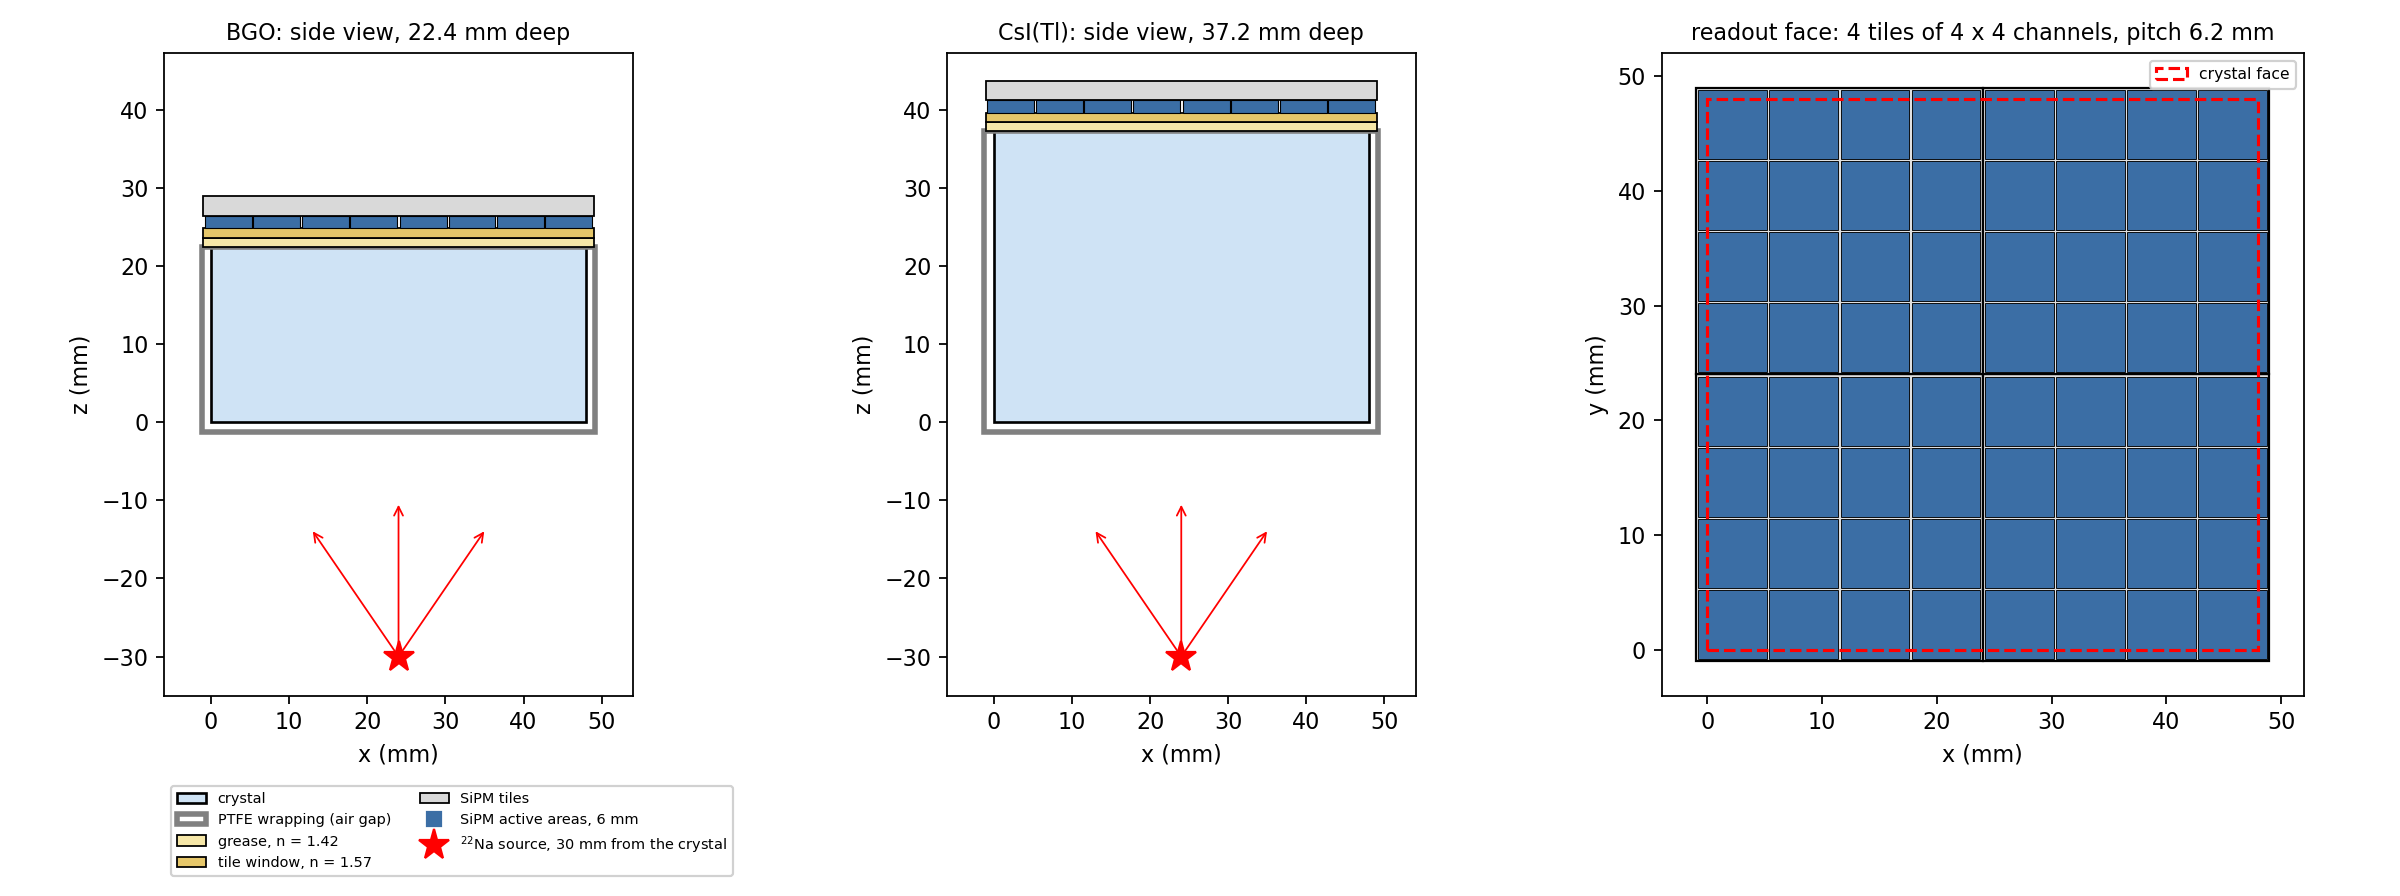
\includegraphics[width=\textwidth]{geometry.png}
\caption{The simulated geometry. Side views of the two crystals with the
wrapping, the grease, the window and the SiPM tiles (the coupling layers
are drawn thicker than they are), and the source; face view of the 64
active areas, grouped in four tiles, with the outline of the crystal.}
\label{fig:geometry}
\end{figure}

\section{The simulation}
\label{sec:sim}

The simulation proceeds in three stages, each writing a file that the next
one reads. The first stage generates the \Na decays, transports the gammas
through the crystal (photoelectric absorption and Compton scattering,
with pair production absorbed locally) and converts each energy deposit into scintillation photons.
The number of photons is the light yield of the crystal, 7600 photons per
MeV for BGO and 54\,000 for \csitl at room temperature, times the
deposited energy, multiplied by one Gaussian factor per decay that
represents the intrinsic resolution of the crystal: 5\% FWHM at 511~keV for
both crystals, scaling as the inverse square root of the energy. The
photons are emitted with the time distribution of the crystal, two components of
300~ns (90\%) and 60~ns (10\%) for BGO and of 730~ns
(64\%) and 3340~ns (36\%) for \csitl, at the wavelength of the emission
maximum, 480~nm for BGO and 550~nm for \csitl. The photons are then transported through the crystal,
its surfaces, the wrapping and the coupling layers until they are absorbed
or reach the active area of a SiPM; the stage records every photon that
arrives there, with its channel, time and wavelength.

The second stage applies the response of the SiPMs. Each recorded photon
produces a photoelectron with the photon detection efficiency of the
device at its wavelength and at the overvoltage of the run, the excess of
the bias voltage over the breakdown voltage. Each photoelectron fires a
cell, which may in turn fire neighbouring cells by optical crosstalk and
produce delayed afterpulses; independently, thermal dark counts fire cells
at random times with the same companions. All these depend on the
overvoltage; Table~\ref{tab:conditions} gives their values. We call
\emph{fired cells} the sum of photoelectrons, crosstalk and afterpulses
produced by the scintillation light, and use the charge of one fired cell,
the gain of the SiPM, as the unit of charge: a recorded charge divided by
it is expressed in \emph{photoelectron equivalents}. The gain of each
channel differs from the nominal one by a Gaussian factor of 5\% rms.
Crosstalk is a branching process: every fired cell, whether fired by a
photon, a thermal carrier or crosstalk, fires a Poisson number of
neighbours, with a mean chosen so that the probability of at least one
companion is the crosstalk probability of the datasheet. The current
pulse of one fired cell is the recharge of the cell through its quenching
resistor, with a time constant of 50~ns, filtered by the input resistance
of the readout in parallel with the 2~nF capacitance of the whole device;
for an input of 50~$\Omega$ the filter has a time constant of 100~ns, and
the pulse peaks 69~ns after the avalanche and falls with 100~ns. The
recharge time is not given by the datasheet and the input resistance is
known only for the Citiroc; the values chosen give the slower of the
plausible pulses, which is the conservative choice for the pile-up of dark
counts.

The third stage applies the readout to the train of fired cells of each
channel. For the Citiroc and the Radioroc2 the train is shaped by a filter
of one differentiating and two integrating stages with the peaking time of
each path, noise is added, a trigger is formed from the discriminators of
the chip, and a peak detector stores the maximum of the shaped signal of
every channel from the trigger until the \emph{hold}, a fixed delay after
the trigger, before the conversion by an ADC. The preamplifiers of the
Radioroc2 are charge-sensitive, so its shaped signal follows the charge of
the pulses; those of the Citiroc amplify the voltage that the current
develops across the 50~$\Omega$ termination, so that its shaper
differentiates the pulse itself and keeps mostly its rising edge. The
electronic noise is 0.1~photoelectron rms on the high-gain path at the
longest shaping of each chip, growing as the inverse square root of the
peaking time; scaled from the datasheet of the Radioroc2 to the 2~nF of our
SiPM it would be about 0.07, and the larger value is kept as a
conservative estimate. The chips hold their output at a fixed level, so
the mean current of the dark counts gives no offset and only its
fluctuations remain. For the digitiser, the charge
that the offline analysis integrates over a window, minus the baseline
measured before it, is computed directly from the times of the fired
cells, and the trigger is formed from the sampled amplitude of each
channel with its noise. The three stages and the parameters of each model
are described in the design document of the simulation.

\section{Operating conditions}
\label{sec:conditions}

The operating conditions are the best compromise found by the simulation
for each readout (Table~\ref{tab:conditions}). They are proposals for the
measurements, and each rests on inputs that the first runs will measure:
the gain, crosstalk and dark-count rate of the SiPMs at room temperature,
which set the thresholds, and, for the digitiser, its noise at the chosen
gain. The simulation assumes the 4~counts per sample of the manual at every
gain; if the noise in counts grows in proportion to the gain, the gain
of 4 brings no advantage over unit gain. The overvoltage of the SiPMs is 3~V for both
ASICs with BGO; with \csitl, whose light is seven times more abundant, it
is lowered to keep the brightest channel within the range of the chip:
to 2.7~V for the Citiroc, whose input saturates at 400~pC, and to 2.0~V for
the Radioroc2, whose low-gain path saturates at 2000 photoelectrons of
unit gain $10^6$. The digitiser operates at 5~V, the setting used so far
on the bench, at a gain of 4, where the simulation places one
photoelectron at 64~ADC counts against the assumed noise of 4~counts per
sample; the pulse of the model would give five times less, and the first
measurement at gains 1, 4 and 8 decides. Both ASICs read the energy on
their low-gain path and calibrate on their high-gain path, each with its
own peaking time: the Citiroc shapes the low gain with its longest peaking
time, 87.5~ns, and the high gain with 25~ns; the Radioroc2 the low gain
with its longest, 1.8~\us, and the high gain with 100~ns. These high-gain
settings are those at which the calibration of Section~\ref{sec:analysis}
fits every channel with the smallest scatter. The digitiser integrates over
1~\us for BGO and 3~\us for \csitl, starting 50~ns before the trigger,
with a baseline measured over the 900~ns before the integration window;
these values minimise the energy resolution in a scan of the window.

\begin{table}[htbp]
\centering
\small
\caption{Operating conditions of the six cases. The detection efficiency
is the photon detection efficiency at the peak of its spectral curve; the
dark-count rate is per channel; the window is the hold of the ASICs and
the integration window of the digitiser. Thresholds in photoelectron
equivalents.}
\label{tab:conditions}
\begin{tabular}{l ccc ccc}
\toprule
 & \multicolumn{3}{c}{BGO} & \multicolumn{3}{c}{\csitl} \\
 & Citiroc & DT2745 & Radioroc2 & Citiroc & DT2745 & Radioroc2 \\
\midrule
overvoltage (V) & 3.0 & 5.0 & 3.0 & 2.7 & 5.0 & 2.0 \\
SiPM gain ($10^6$) & 2.8 & 4.7 & 2.8 & 2.5 & 4.7 & 1.9 \\
detection efficiency & 0.52 & 0.54 & 0.52 & 0.50 & 0.54 & 0.41 \\
crosstalk probability & 0.088 & 0.195 & 0.088 & 0.070 & 0.195 & 0.041 \\
dark-count rate (MHz) & 4.3 & 4.4 & 4.3 & 4.1 & 4.4 & 3.3 \\
shaping, high/low gain (ns) & 25/87.5 & --- & 100/1800 & 25/87.5 & --- & 100/1800 \\
window (ns) & 300 & 1000 & 3560 & 500 & 3000 & 3560 \\
trigger & single, 8 & two, 11 & charge, 30 & single, 8 & two, 9 & charge, 20 \\
\bottomrule
\end{tabular}
\end{table}

The trigger differs between the readouts. The Citiroc triggers when one
channel crosses the threshold of its fast discriminator, which follows a
shaper of 15~ns. The digitiser triggers when two channels cross the
threshold within 100~ns, a coincidence that we call a majority of two.
The Radioroc2 triggers on its charge discriminator, which reads the
low-gain shaped signal of each channel. In each case the threshold is the
lowest one at which every 511~keV photopeak event triggers (an efficiency
of at least 0.995) while the dark counts, alone, trigger less than once per
millisecond at 95\% confidence, on a sample of 1500 decays with no energy
deposit. At room temperature this second condition is the restrictive
one: a dark count with three or four crosstalk companions occurs in some
channel in most microseconds, and thresholds of a few photoelectrons
trigger on it. For BGO with the Citiroc no threshold of the scan meets
both conditions: at 8 photoelectron equivalents two decays of the sample
trigger, 0.6~kHz with an upper limit of 1.9~kHz, and at 10 the photopeak
loses 2\% of its events; 8 is kept, and a larger sample of decays will
decide.

\section{Analysis}
\label{sec:analysis}

The analysis treats the simulated files as it will treat the measured ones,
and uses the record of the simulation only to select the events and to
follow the light from the crystal to the readout.

\emph{Calibration.} Each readout is calibrated with its own data only, on
the dark counts recorded without source. For the ASICs, every crossing of
the discriminator of a channel at half a photoelectron holds the high gain
of that channel at the maximum of the pulse that crossed, the delay of
the hold being the one that a scan on the bench would choose; at the short
peaking time of the high gain the dark counts do not pile up under the
held value. The spectrum shows the peaks of 1, 2 and 3 photoelectrons, the
higher ones from crosstalk, on a continuum of pile-up. The peaks are
located as the minima of the second derivative of the smoothed histogram,
which resolves a peak that is only a shoulder on the tail of the previous
one, and the gain and the zero of the high gain are the slope and the
intercept of the straight line through their positions against the number
of photoelectrons. The zero of the low gain is its mean value in the
channels whose discriminator did not fire, on dark-count events triggered
in the same way with the settings of the run. The gain of the low gain is
the high-gain one times the ratio of the two paths, which the
charge-injection input of each chip measures; the simulation assumes this
ratio known. The injected charge arrives at once, while that of an
avalanche is spread over its pulse, so that at a short shaping the high
gain responds less to an avalanche than to the same injected charge; the
measured ratio must be corrected for this with the measured shape of the
pulse. For the digitiser, every record contains tens of dark pulses per
channel; the waveform is filtered with the sampled pulse of one fired cell
(a matched filter) after subtracting the mean of the four preceding
samples, the local maxima of the filtered waveform are the pulse
amplitudes, and the position of the one-photoelectron peak of each
channel, from a Gaussian fit, is its gain. The fitted gains differ from
the true ones by a factor common to all channels, which the energy
calibration absorbs.

\emph{Energy.} The charge of each channel in photoelectron equivalents is,
for the ASICs, the low-gain value minus its zero divided by its gain, and
for the digitiser the integrated charge divided by the gain times the area
of the pulse over its height. The energy of an event is the sum of the 64
channels. In a channel that receives no light the peak detector stores the
largest dark pulse or noise excursion within the hold, so the zero of the
low gain lies above the electronic pedestal, by 2.0 to 2.4 photoelectron
equivalents per channel. This offset is not exactly additive, since in a
channel that receives light a dark pulse changes the stored maximum only
when it falls on top of the signal. A straight line through the positions
of the 511 and 1275~keV peaks converts the sum into keV and absorbs the
residual offset. The 511~keV peak is fitted with a Gaussian on a linear
background, and the energy resolution is its FWHM divided by its
position. Each case uses 10\,000 decays, with 1341 photopeak events for
BGO and 762 for \csitl; the resolution is known to 0.2 points and the
1275~keV peak, with fewer events, only roughly. A run of 50\,000 decays
will follow.

\emph{Light.} The events in which one 511~keV gamma deposits its full
energy in the crystal, without any deposit of the 1275~keV gamma, are
selected from the record of the simulation. On these events we count the photons emitted, the
photons that reach the active areas of the SiPMs, the photoelectrons and
the fired cells, the last two from a replay of the SiPM response without
dark counts, and we take the recorded charge at 511~keV in photoelectron
equivalents from the energy calibration. The ratios between consecutive
quantities are the collection efficiency of the crystal and its coupling,
the detection efficiency at the emission wavelength, and the
fraction of the photoelectrons that the readout records.

\emph{Resolution.} On the same events, the relative width of each quantity
(half the interval between its 16th and 84th percentiles divided by its
median, multiplied by 2.355 to compare with a FWHM) separates the
contributions to the energy resolution. The width of the number of
photoelectrons contains the intrinsic resolution of the crystal and the
statistics of the light collection and detection; the difference in
quadrature with the intrinsic 5\% is the statistical contribution. The
difference in quadrature between the widths of the fired cells and of the
photoelectrons is the contribution of crosstalk and afterpulses; that
between the recorded energy and the fired cells is the contribution of the
readout, which includes the dark counts, the electronic noise, the
fluctuation of the fraction of the light that the shaping keeps and the
zero level.

\section{BGO}
\label{sec:bgo}

A 511~keV deposit in BGO emits 3885 photons, of which 3254 (84\%) reach the
SiPMs and 1585 become photoelectrons at 3~V, 1634 at 5~V. The width of the
number of photoelectrons is 7.7\% FWHM, the intrinsic 5\% and a
statistical term of 5.8\%, the value expected from 1585 photoelectrons.

\subsection{Citiroc 1A}

The single-channel threshold of 8 photoelectron equivalents triggers on
every 511~keV event but only on 69\% of the deposits between 200 and
300~keV, while the dark counts trigger at about 0.6~kHz
(Figure~\ref{fig:bgo_citiroc}). The fast shaper of the trigger follows the
voltage preamplifier and sees the rising edges of the pulses, so that the
slow BGO light reaches a low amplitude in it compared with a dark pulse
and its crosstalk companions. The high gain at 25~ns shows the peaks of 1,
2 and 3 photoelectrons; the fitted gain is 0.943 of the true one and
follows it channel by channel with a scatter of 2.2\%, against the 5\%
spread of the gains. The low gain at 87.5~ns keeps 0.29 of a 300~ns light
pulse: the recorded charge at 511~keV is 570 photoelectron equivalents,
0.36 of the photoelectrons, the crosstalk adding to the stored amplitude.
The energy resolution is 11.1\% FWHM. The readout contributes 8.5\%, more
than the statistics: the fraction of the light that the shaping keeps
depends on the times of arrival of the photoelectrons and fluctuates from
event to event. The ratio of the 1275 and 511~keV peak positions is 2.57,
and the energy scale has an offset of 25~keV.

\begin{figure}[htbp]
\centering
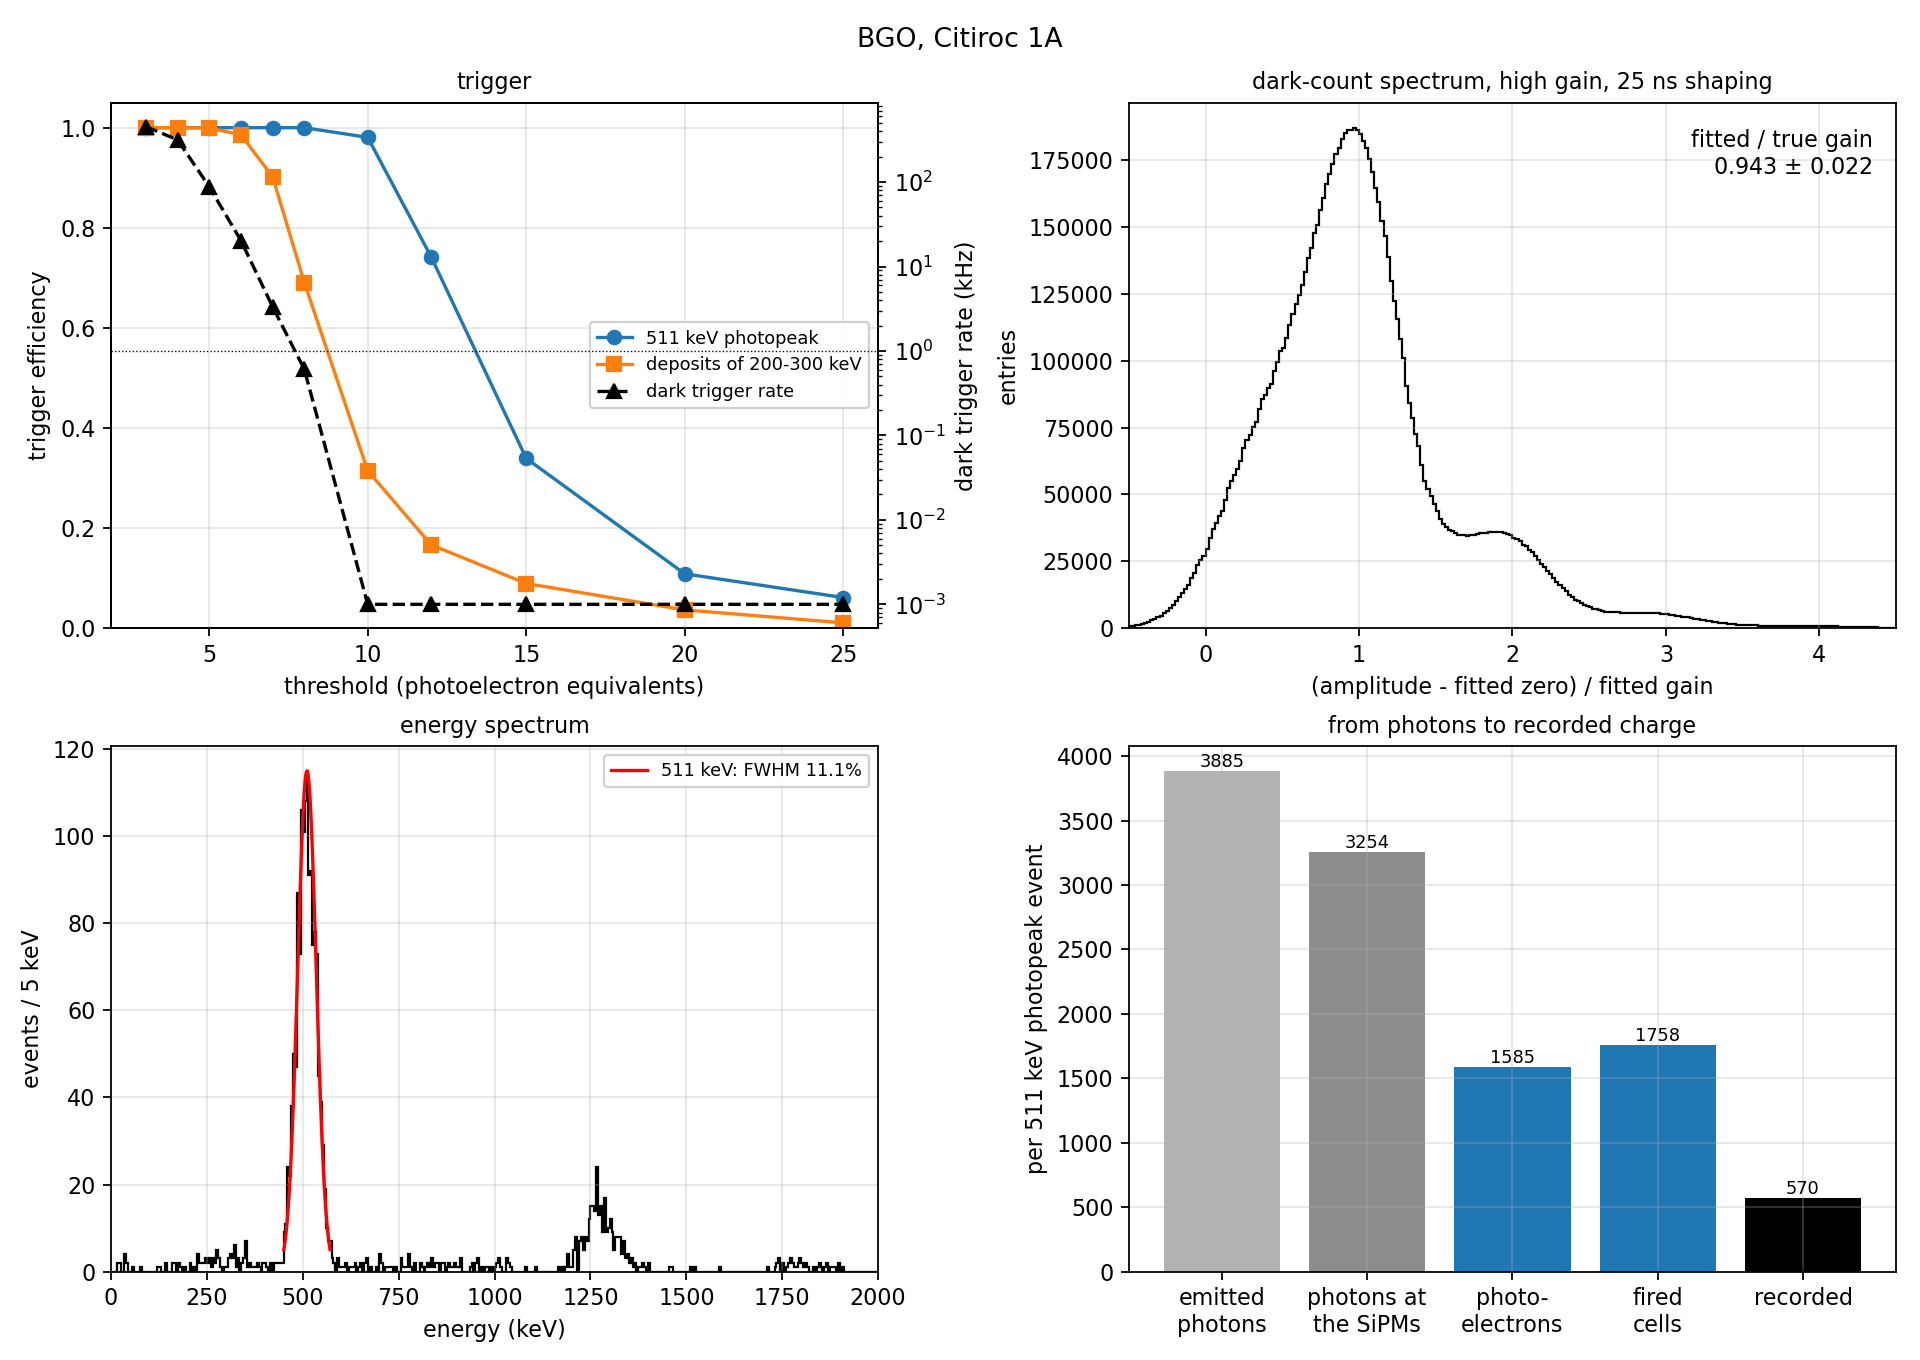
\includegraphics[width=\textwidth]{case_bgo_citiroc.png}
\caption{BGO read by the Citiroc~1A. Top left: trigger efficiency for the
511~keV photopeak and for deposits of 200 to 300~keV, and dark trigger
rate, against the threshold; rates below the sensitivity of the sample
are drawn at $10^{-3}$~kHz. Top right: spectrum of the dark counts on the
high gain at 25~ns, all channels, each calibrated with its fitted zero and
gain. Bottom left:
calibrated energy spectrum with the fit of the 511~keV peak. Bottom right:
photons emitted, photons at the SiPMs, photoelectrons, fired cells and
recorded charge per 511~keV photopeak event.}
\label{fig:bgo_citiroc}
\end{figure}

\subsection{DT2745 digitiser}

The threshold of 704~ADC counts, 11 photoelectrons at the assumed height of
one photoelectron, with a majority of two triggers on every 511~keV event
and on 99.7\% of the deposits between 200 and 300~keV; no decay without
deposit triggers in the sample, which bounds the dark trigger rate below
0.4~kHz (Figure~\ref{fig:bgo_dig}). At gain 4 the matched filter separates
the single-photoelectron peaks cleanly; the fitted gain is 1.031 of the
true one with a scatter of 0.2\% between channels. The integration window
of 1~\us records nearly the whole light pulse, so that the recorded
charge, 1908 photoelectron equivalents, exceeds the 1634 photoelectrons by
the crosstalk (19.5\% at 5~V) and the afterpulses. The energy resolution
is 9.2\% FWHM. Crosstalk and afterpulses contribute 3.2\%, and the readout
4.6\%: the integration window collects 280 dark counts on average over the
64 channels, with their crosstalk, and their fluctuation adds to the
width. The ratio of the peak positions is 2.47.

\begin{figure}[htbp]
\centering
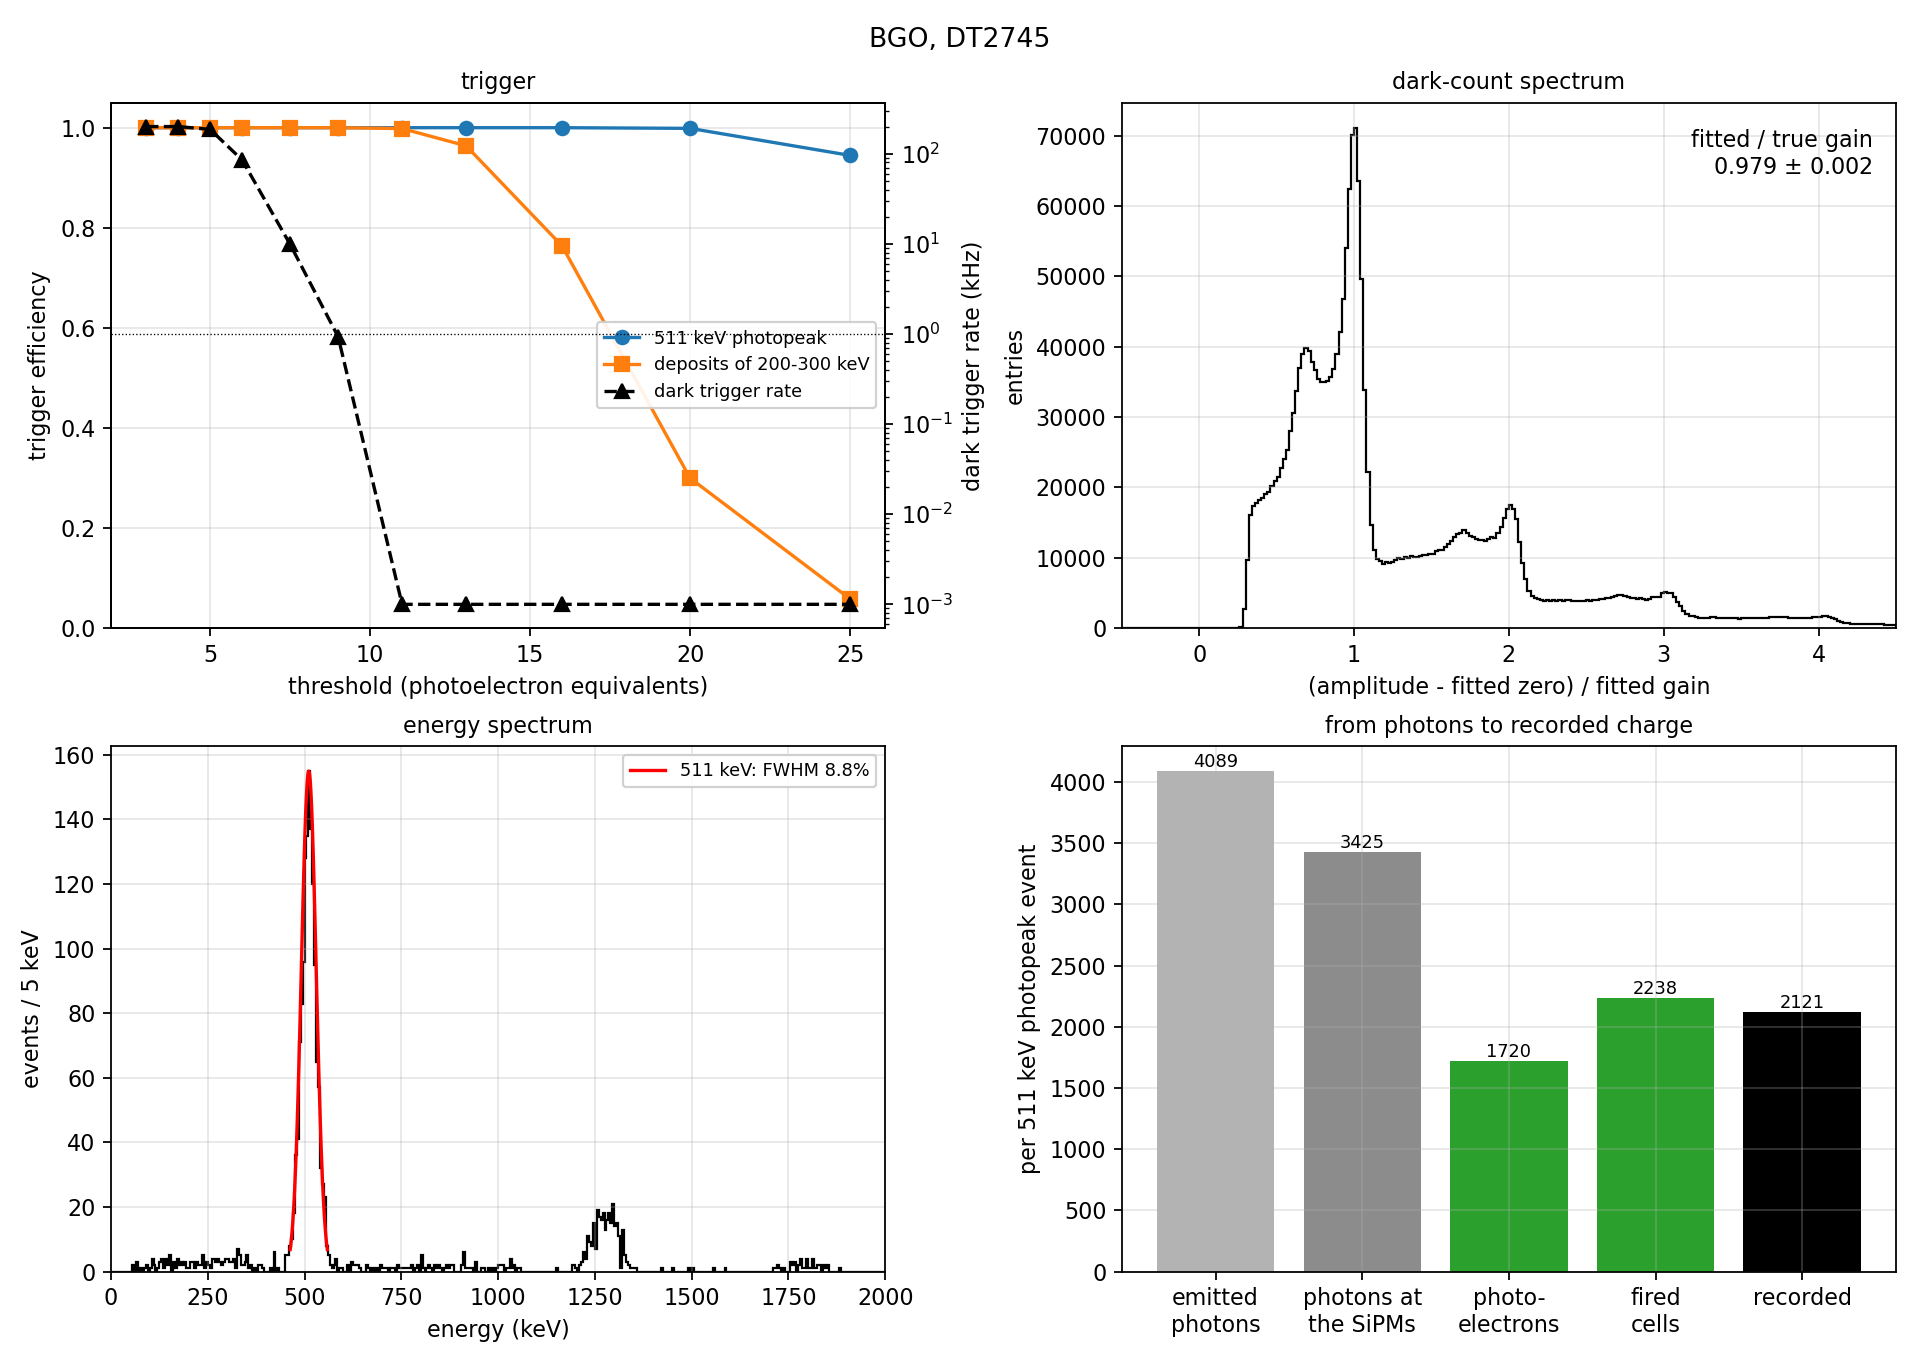
\includegraphics[width=\textwidth]{case_bgo_digitiser.png}
\caption{BGO read by the DT2745 digitiser at gain 4 and 5~V of
overvoltage. Panels as in Figure~\ref{fig:bgo_citiroc}; the dark-count
spectrum is that of the matched-filter amplitudes.}
\label{fig:bgo_dig}
\end{figure}

\subsection{Radioroc2}

The charge trigger at 30 photoelectron equivalents triggers on every
511~keV event and on 85\% of the deposits between 200 and 300~keV; it
requires one channel above threshold, and the brightest channel of such a
deposit is sometimes below it. No decay without deposit triggers, which
bounds the dark trigger rate below 0.3~kHz (Figure~\ref{fig:bgo_rr}). At
the shaping of 1.8~\us no single-photoelectron peak exists, because the
dark counts pile up within the shaping time; at 100~ns on the high gain
the peaks of 1, 2 and 3 photoelectrons are clear, the fitted gain is 0.959
of the true one and follows it with a scatter of 3.6\%. The spectrum also
holds a population at zero, crossings of the time discriminator with no
signal on the high gain, which the fit leaves out and which remains to be
understood. The long shaping keeps almost all the light: the recorded
charge, 1758 photoelectron equivalents, is 1.11 times the photoelectrons.
The zero of the low gain adds up to 156 photoelectron equivalents over the
64 channels; the energy scale keeps an offset of 35~keV and a ratio of the
peak positions of 2.60, which the two-point calibration absorbs. The
energy resolution is 9.2\% FWHM, with a readout contribution of 4.7\%.

\begin{figure}[htbp]
\centering
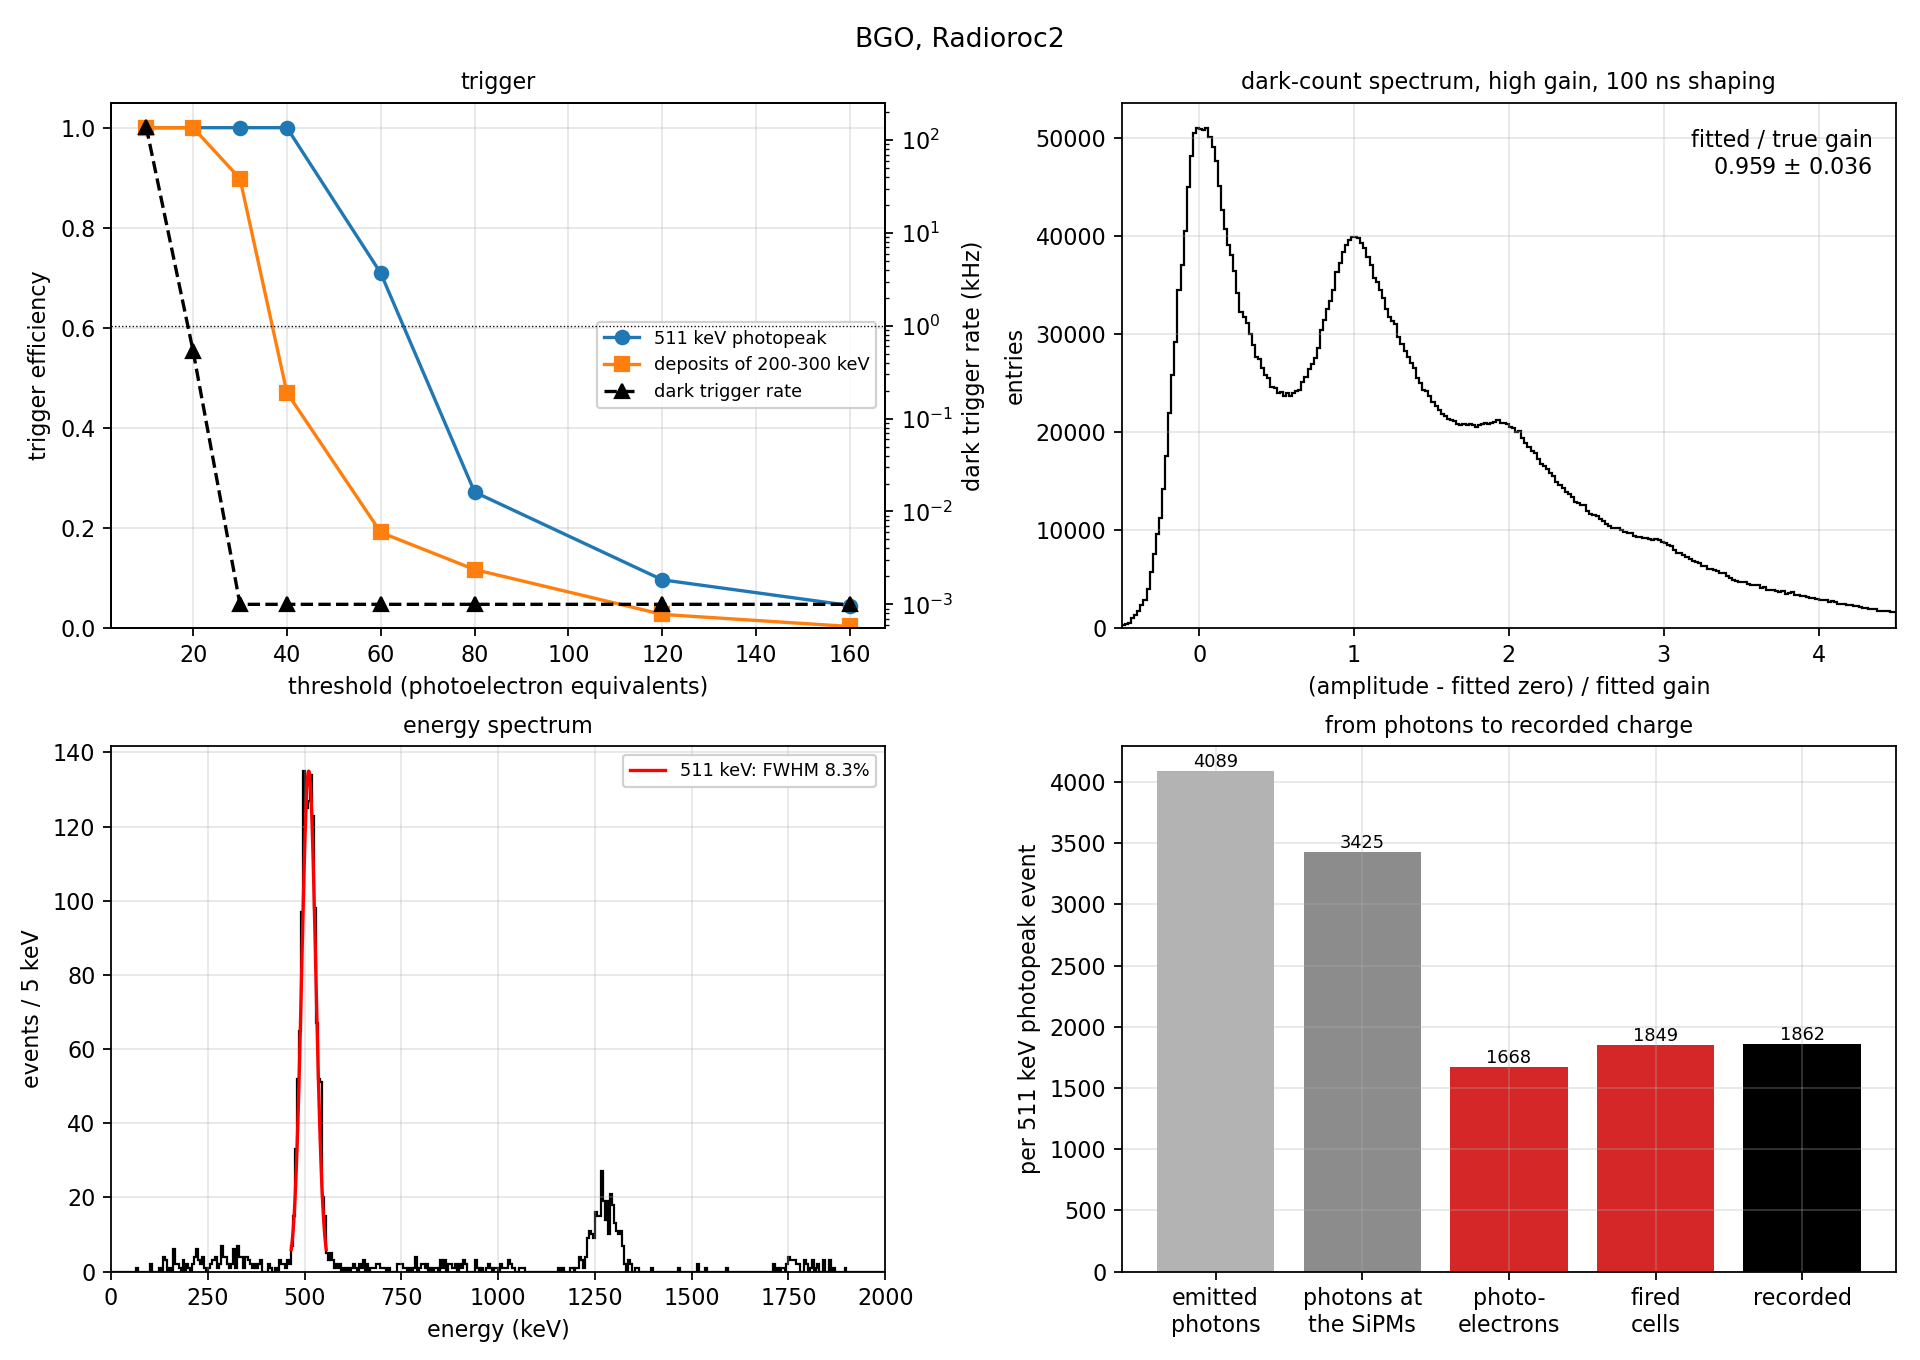
\includegraphics[width=\textwidth]{case_bgo_radioroc.png}
\caption{BGO read by the Radioroc2 at 1.8~\us of shaping. Panels as in
Figure~\ref{fig:bgo_citiroc}; the dark-count spectrum is that of the high
gain at 100~ns of shaping.}
\label{fig:bgo_rr}
\end{figure}

\section{\csitl}
\label{sec:csi}

A 511~keV deposit in \csitl emits 27\,600 photons, of which 23\,210 (84\%)
reach the SiPMs. The detection efficiency at the 550~nm emission is lower
than at 480~nm, and the number of photoelectrons depends on the
overvoltage: 7214 at 2.0~V, 8825 at 2.7~V and 9528 at 5~V. The
statistical contribution to the width is therefore 2.7 to 2.9\%, about half
of the intrinsic 5\%.

\subsection{Citiroc 1A}

The single-channel threshold of 8 photoelectron equivalents triggers on
every 511~keV event and on 96\% of the deposits between 200 and 300~keV,
at a dark trigger rate of 0.1~kHz (Figure~\ref{fig:csi_citiroc}). The
calibration is that of BGO, with a fitted gain of 0.941 of the true one
and a scatter of 1.8\% between channels. The low gain at 87.5~ns keeps a
tenth of a light pulse that lasts microseconds: the recorded charge is
1020 photoelectron equivalents, 0.12 of the 8825 photoelectrons. The
energy resolution is 8.3\% FWHM, of which the readout contributes 6.4\%,
the largest term. The ratio of the peak positions is 2.56.

\begin{figure}[htbp]
\centering
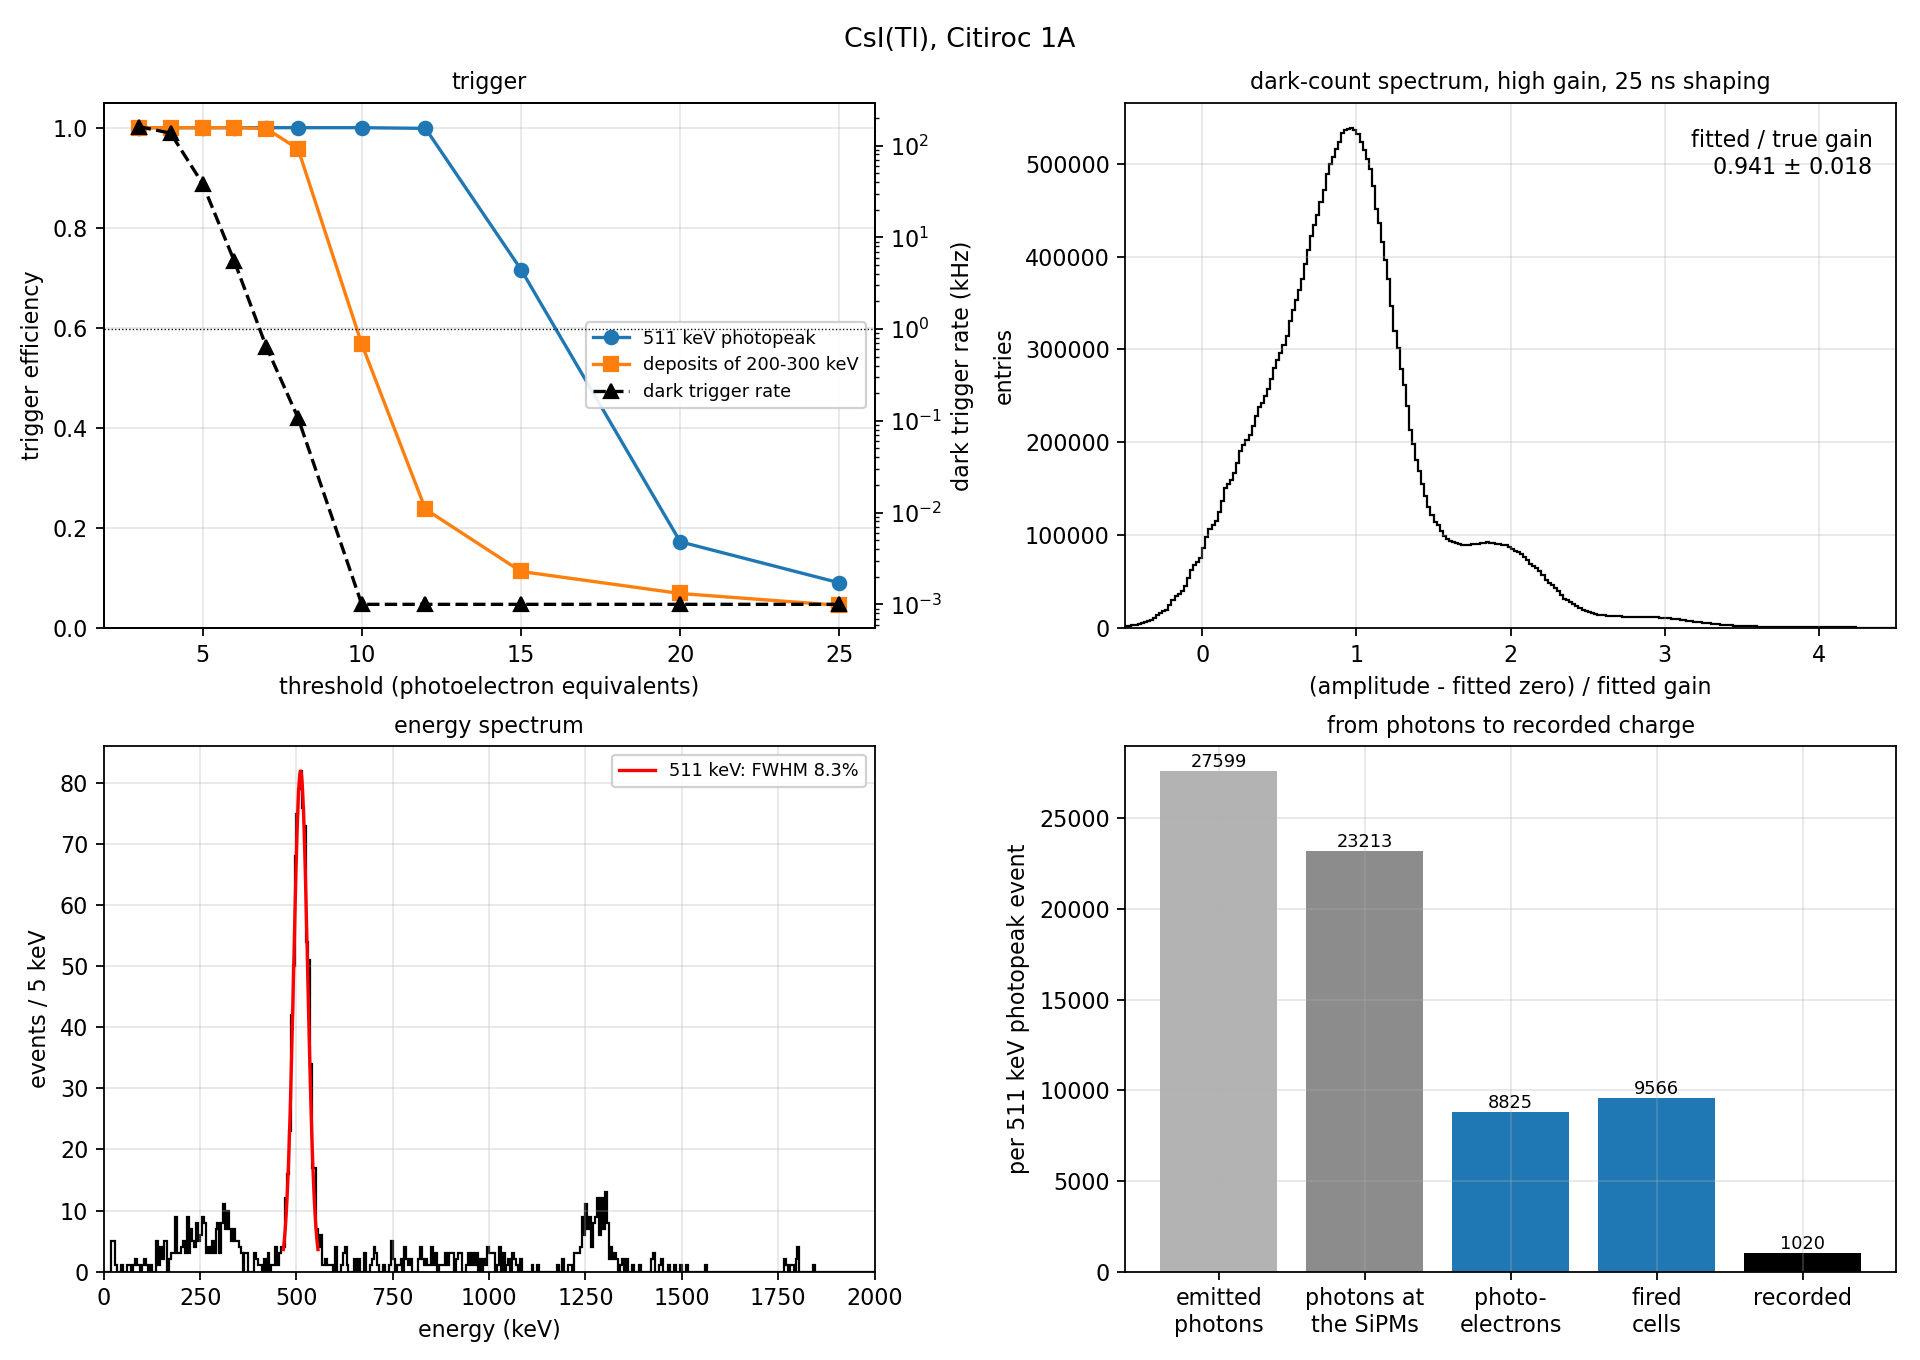
\includegraphics[width=\textwidth]{case_csitl_citiroc.png}
\caption{\csitl read by the Citiroc~1A. Panels as in
Figure~\ref{fig:bgo_citiroc}.}
\label{fig:csi_citiroc}
\end{figure}

\subsection{DT2745 digitiser}

The threshold of 576~ADC counts, 9 photoelectrons, with a majority of two
triggers on every event of the two classes; eight of the 1500 decays
without deposit trigger, 0.5~kHz with an upper limit of 1.0~kHz
(Figure~\ref{fig:csi_dig}). The calibration is that of BGO. The
integration window of 3~\us holds most of both light components: the
recorded charge is 10\,088 photoelectron equivalents, 1.06 times the 9528
photoelectrons, the crosstalk compensating the light that falls after the
window. The energy resolution is 6.2\% FWHM. The window collects 850 dark
counts on average, and the readout contributes 1.6\%.

\begin{figure}[htbp]
\centering
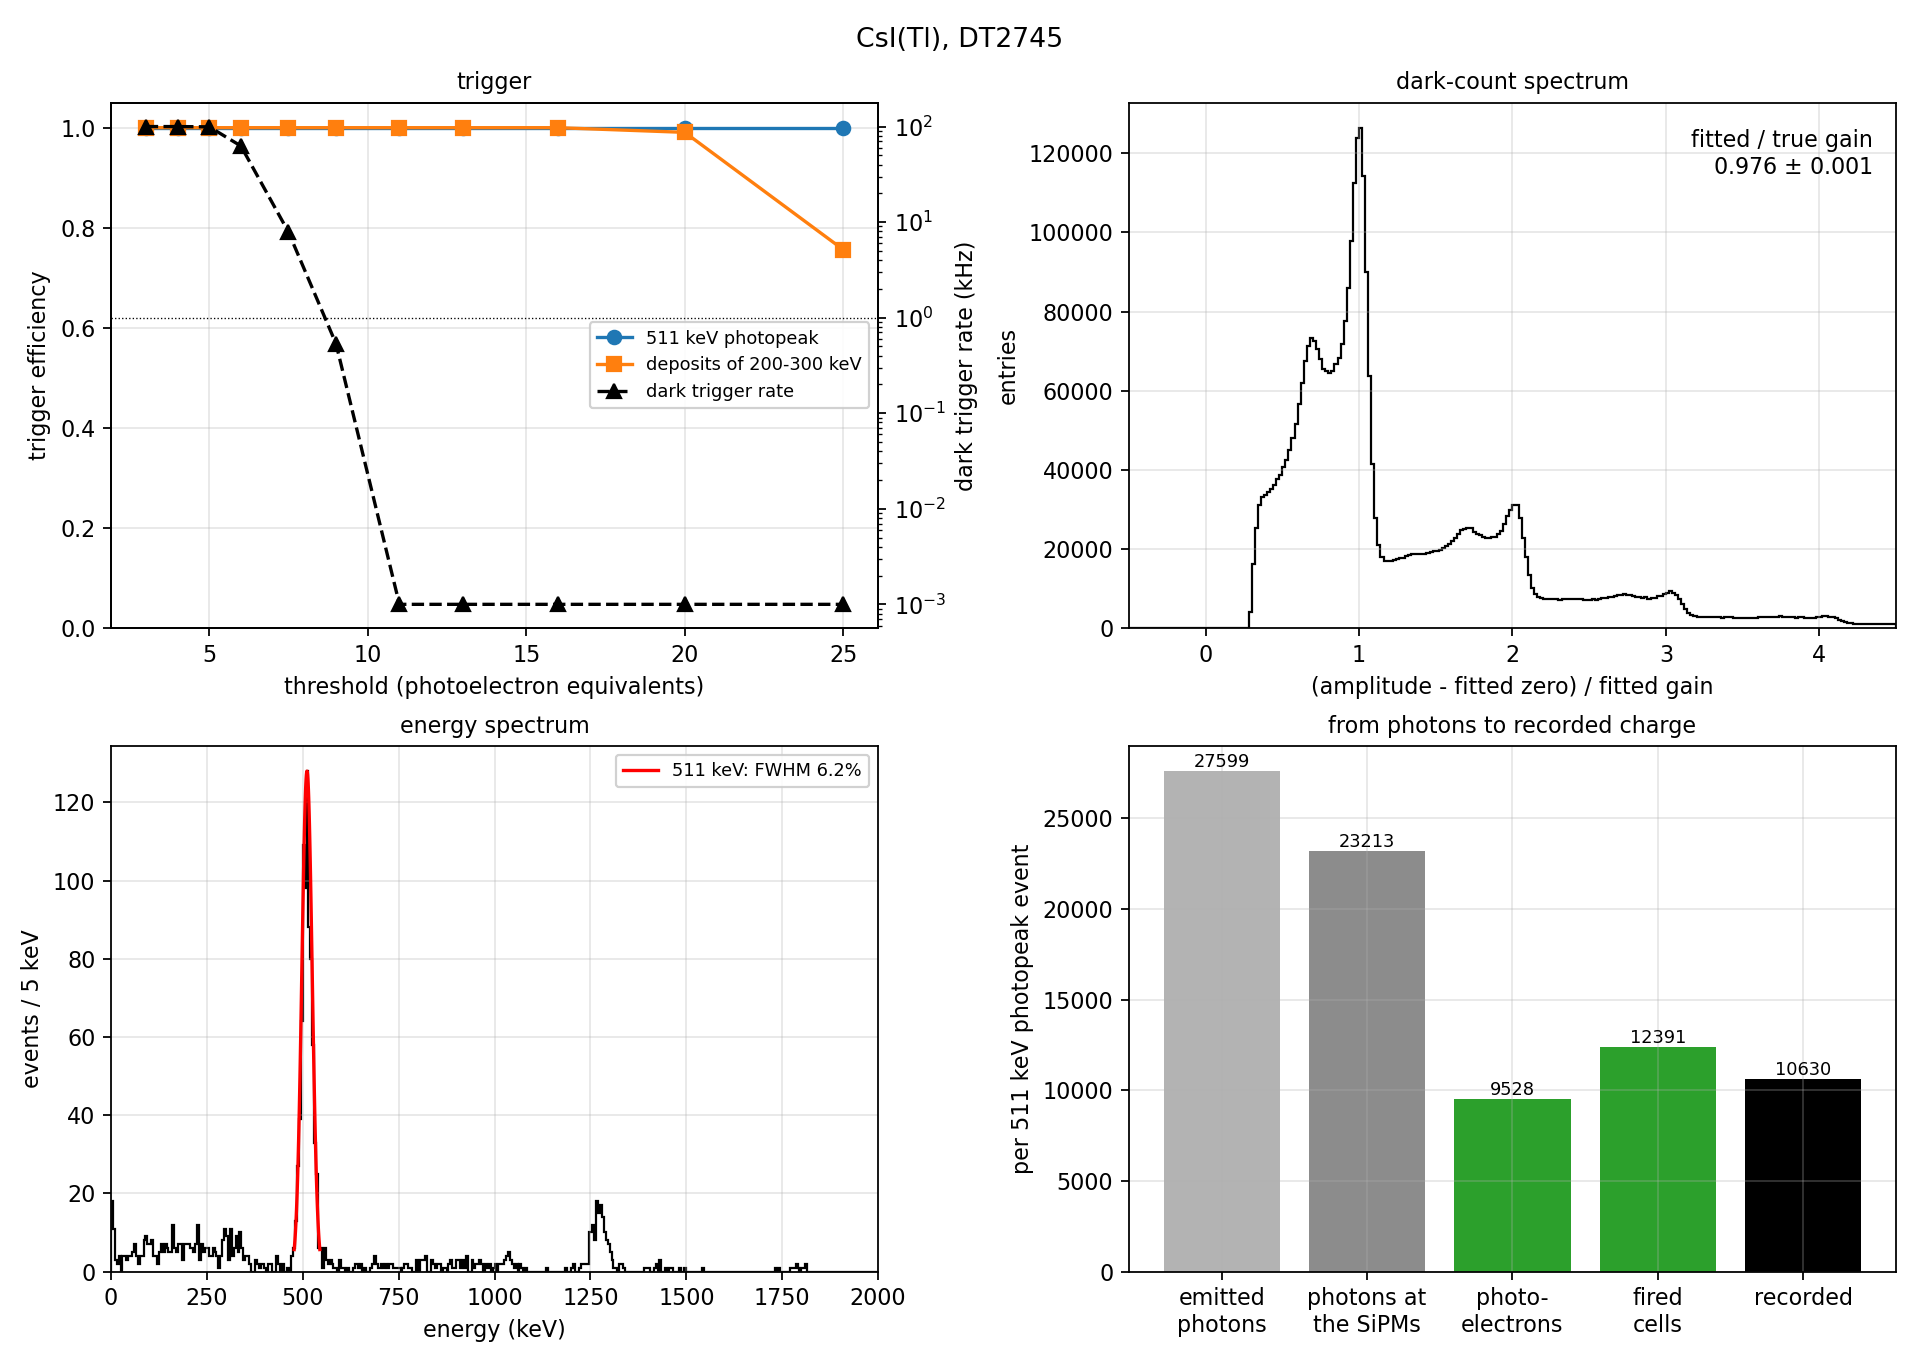
\includegraphics[width=\textwidth]{case_csitl_digitiser.png}
\caption{\csitl read by the DT2745 digitiser. Panels as in
Figure~\ref{fig:bgo_dig}.}
\label{fig:csi_dig}
\end{figure}

\subsection{Radioroc2}

The charge trigger at 20 photoelectron equivalents triggers on every event
of the two classes, and no decay without deposit triggers
(Figure~\ref{fig:csi_rr}). The calibration at 100~ns gives a fitted gain
of 0.965 of the true one, with a scatter of 3.1\%. At 2.0~V the brightest
channel holds 970 photoelectron equivalents in one photopeak event of a
hundred, below the ceiling of the low gain, 1075 at this SiPM gain, but
the overvoltage yields 18\% fewer photoelectrons than 2.7~V. The shaping
of 1.8~\us keeps 0.71 of a \csitl light pulse: the recorded charge is 5531
photoelectron equivalents, 0.77 of the photoelectrons. The energy
resolution is 6.0\% FWHM, with a readout contribution of 2.6\%; the ratio
of the peak positions is 2.52.

\begin{figure}[htbp]
\centering
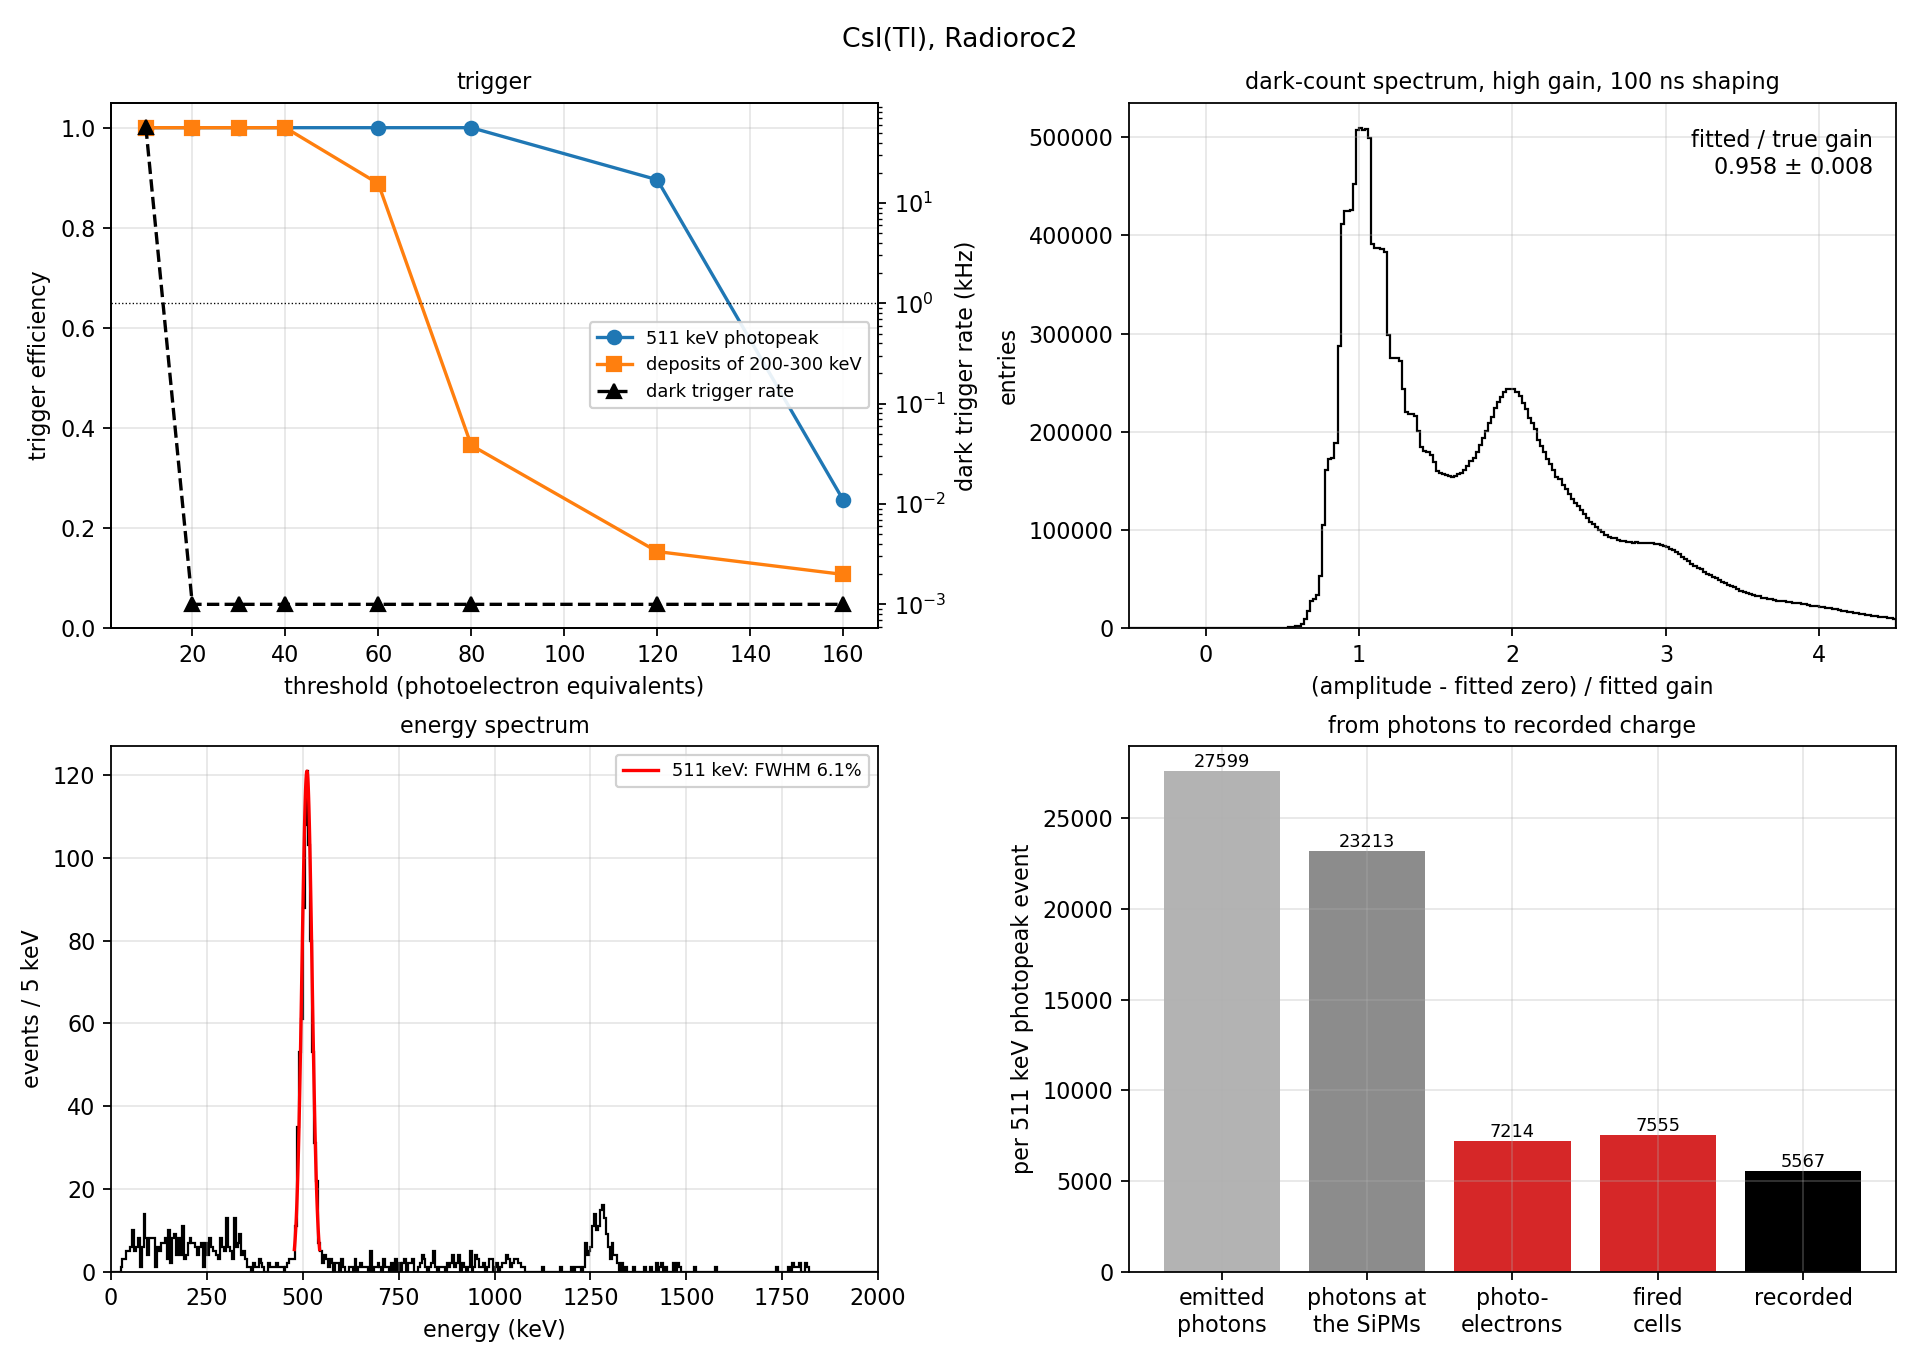
\includegraphics[width=\textwidth]{case_csitl_radioroc.png}
\caption{\csitl read by the Radioroc2. Panels as in
Figure~\ref{fig:bgo_rr}.}
\label{fig:csi_rr}
\end{figure}

\section{Comparison}
\label{sec:comparison}

Figure~\ref{fig:resolution} gathers the energy resolutions and their
decomposition. For BGO the three readouts span 9.2 to 11.1\%, for \csitl
6.0 to 8.3\%, and in every case the intrinsic resolution of the crystal
and the statistics of the photoelectrons account for most of the width.
For BGO the statistical term, 5.8\%, is as large as the intrinsic one,
because the crystal produces few photons; for \csitl it is half of it.
The readout term is largest for the Citiroc, whose voltage preamplifier
and short shaping record a small and fluctuating fraction of a long light
pulse, 8.5\% for BGO and 6.4\% for \csitl. The digitiser and the Radioroc2
come close to each other: for BGO both reach 9.2\%, the digitiser losing
to its crosstalk at 5~V what it gains by integrating the whole pulse, and
for \csitl the readout term is 1.6\% for the digitiser and 2.6\% for the
Radioroc2, whose lower overvoltage yields fewer photoelectrons; the
resolutions, 6.2 and 6.0\%, are equal within their uncertainty.

\begin{figure}[htbp]
\centering
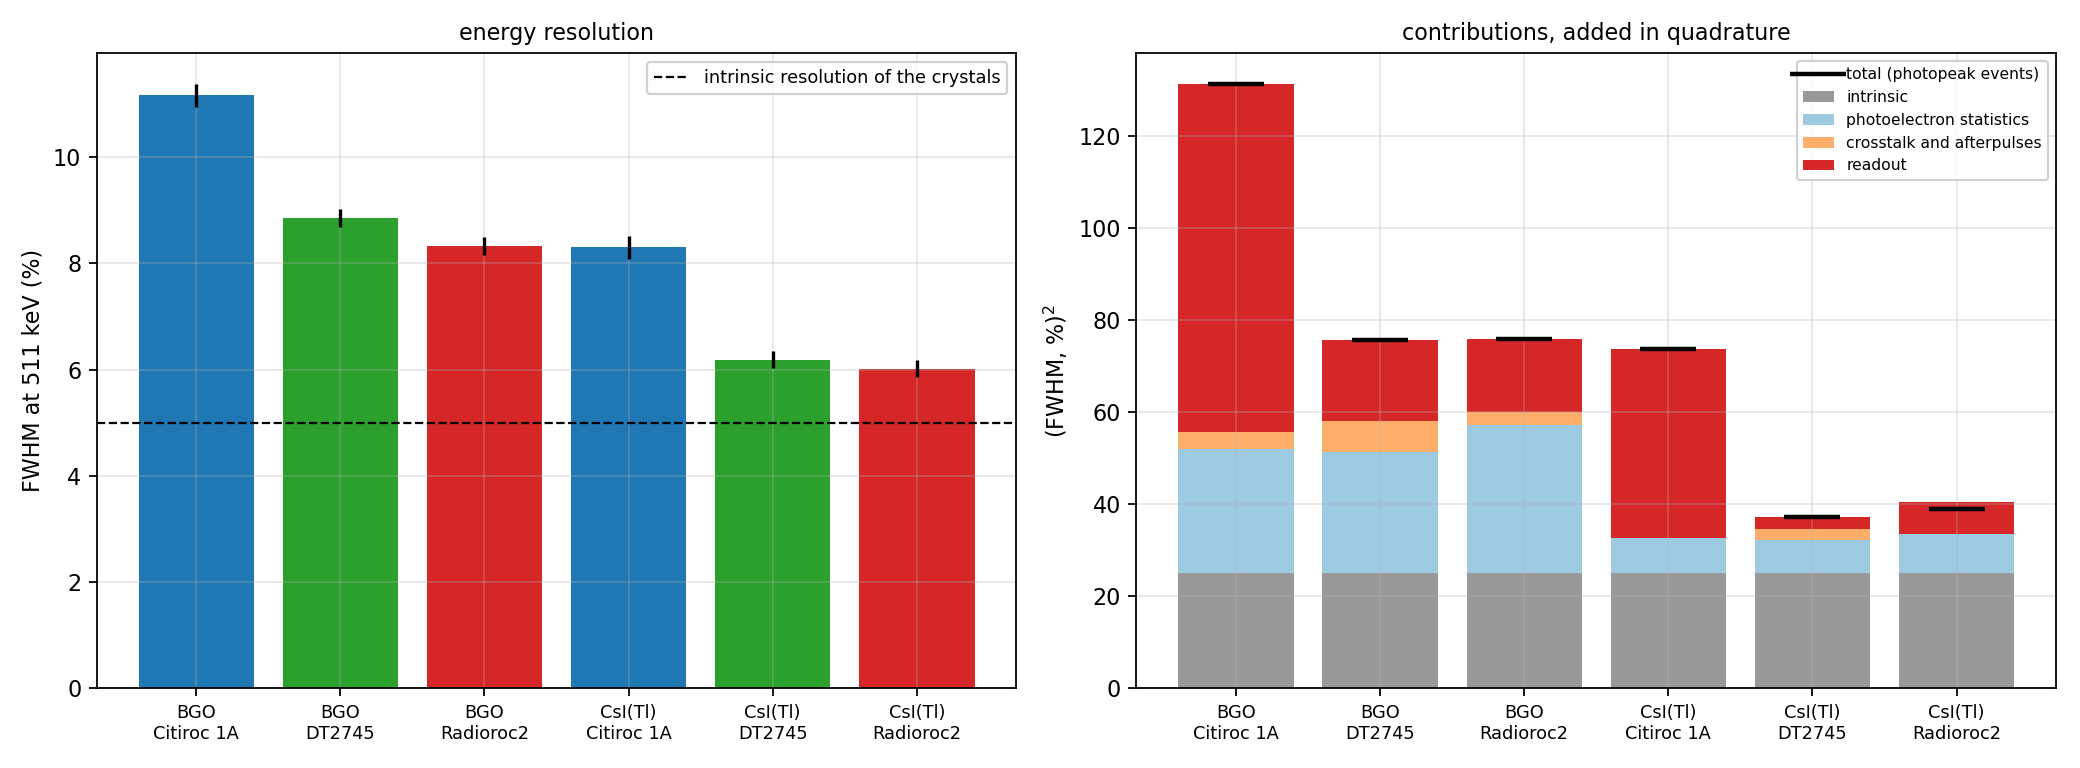
\includegraphics[width=\textwidth]{compare_resolution.png}
\caption{Left: energy resolution at 511~keV of the six cases, with the
intrinsic resolution of the crystals. Right: the squares of the
contributions to the width of the photopeak events, stacked; the bar marks
the total.}
\label{fig:resolution}
\end{figure}

Figure~\ref{fig:light} shows the chain from photons to recorded charge.
The collection efficiency, 0.84, is a property of the crystal and its
coupling and is common to the three readouts. The detection efficiency at
the emission wavelength is 0.49 to 0.50 for BGO and 0.31 to
0.41 for \csitl, depending on the overvoltage. The fraction of the
photoelectrons recorded spans an order of magnitude: 0.12 for \csitl and
0.36 for BGO with the Citiroc, 0.77 and 1.11 with the Radioroc2 and above
one with the digitiser, whose integral includes the crosstalk. The number
of photoelectrons sets the statistical limit; the recorded fraction sets
how close a readout comes to it.

\begin{figure}[htbp]
\centering
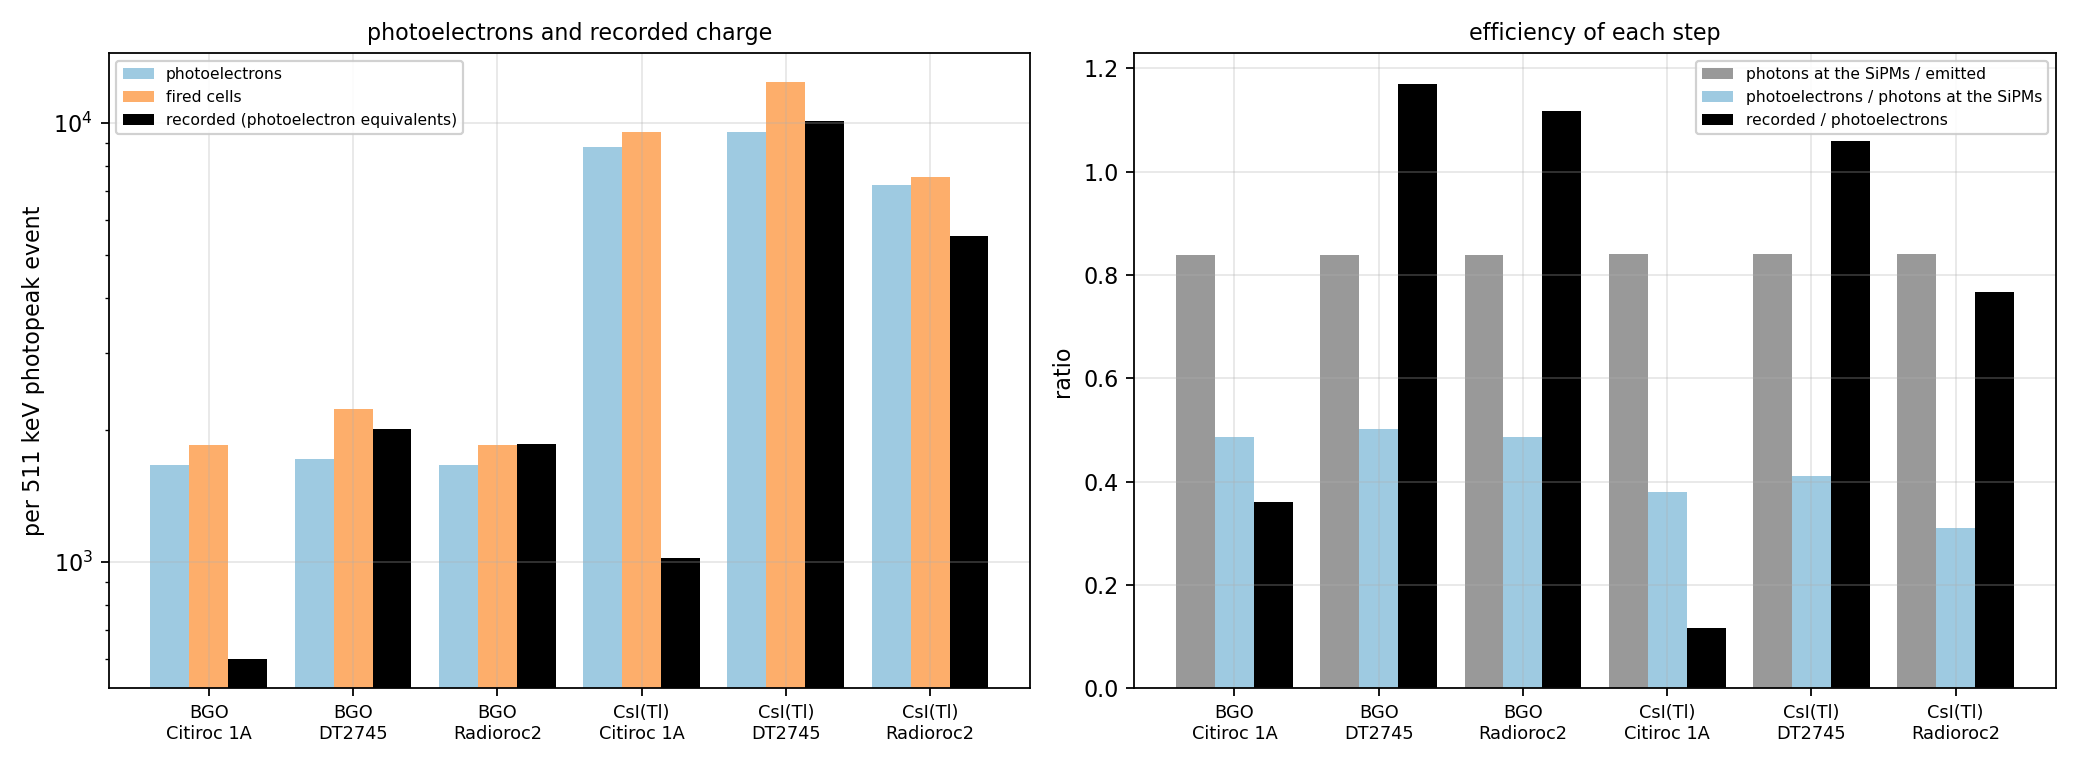
\includegraphics[width=\textwidth]{compare_light.png}
\caption{Left: photoelectrons, fired cells and recorded charge per 511~keV
photopeak event. Right: collection efficiency, detection efficiency and
fraction of the photoelectrons recorded.}
\label{fig:light}
\end{figure}

Figure~\ref{fig:channels} shows the distributions of the brightest and of
the least illuminated channel in the photopeak events, the two ends of the
dynamic range that a position measurement needs. In BGO the brightest
channel holds a median of 23 photoelectron equivalents with the Citiroc,
64 with the Radioroc2 and 73 with the digitiser, and the least illuminated
one 1 to 9; in \csitl the brightest channel reaches 1800 photoelectron
equivalents in one event of a hundred with the digitiser, which its range
holds, and 970 with the Radioroc2, near the limit of its low gain.

\begin{figure}[htbp]
\centering
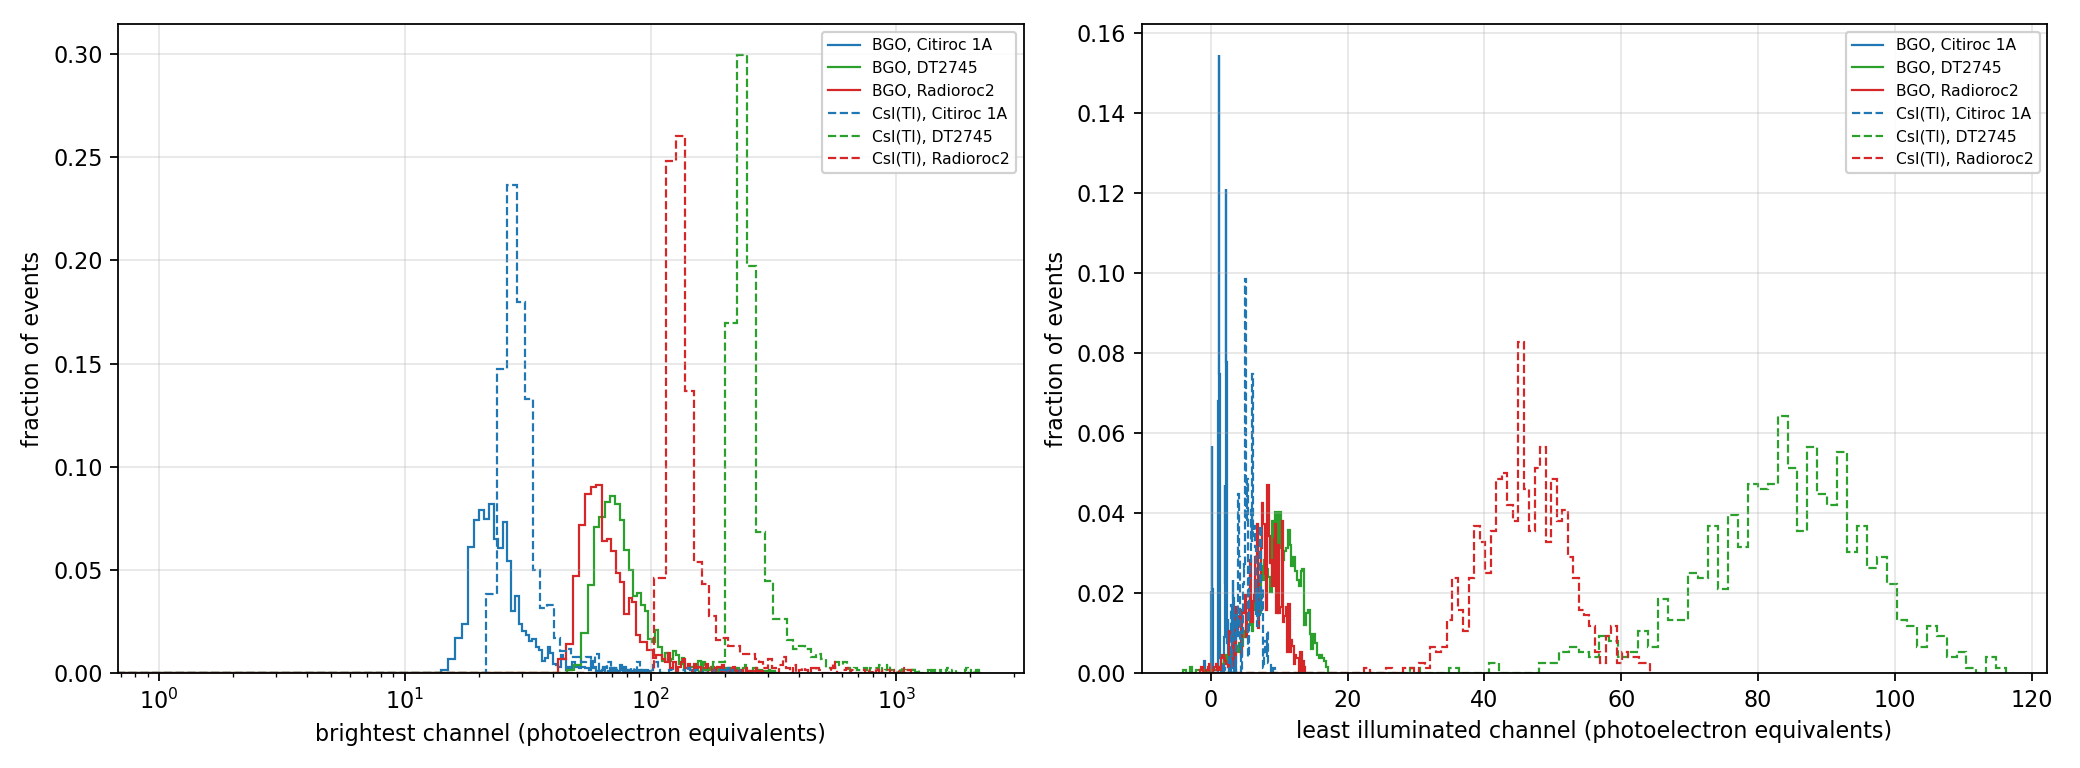
\includegraphics[width=\textwidth]{compare_channels.png}
\caption{Brightest (left) and least illuminated (right) channel of the
511~keV photopeak events, zero level subtracted, in photoelectron
equivalents. Solid lines BGO, dashed lines \csitl.}
\label{fig:channels}
\end{figure}

\section{Conclusions}
\label{sec:conclusions}

At room temperature the three readouts measure the energy of a 511~keV
deposit with resolutions of 9.2 to 11.1\% FWHM for BGO and 6.0 to 8.3\%
for \csitl. The resolution is limited by the crystal, through its
intrinsic resolution and, for BGO, its low light yield; the readout adds a
term of 6 to 9\% for the Citiroc and of 2 to 5\% for the digitiser and the
Radioroc2. The dark counts of the SiPMs, about 4~MHz per channel, shape the
operation of every readout: they set the trigger thresholds at 8 to 11
photoelectrons, add to the width through the integration window of the
digitiser and the zero level of the peak detectors, and determine how the
gain can be calibrated. In the simulation each readout calibrates on its
own dark counts: the digitiser at gain 4 with a matched filter, provided
its noise in counts does not grow with the gain and one photoelectron is
as high as assumed, and the two ASICs on their high-gain path at a short
shaping, 25~ns for the Citiroc and 100~ns for the Radioroc2, whose gain is
transferred to the low-gain path by the ratio that charge injection
measures. The Citiroc, with its voltage-sensitive preamplifiers, keeps the
smallest fraction of the light and triggers least efficiently on BGO
deposits below 300~keV. The first measurements decide whether these
proposals stand: the noise of the digitiser and the height of one
photoelectron at gains 1, 4 and 8, the shape of the SiPM pulse, the noise
of the ASICs with the SiPMs biased below breakdown, the single-photoelectron
spectra, the dark-count rate and crosstalk of the SiPMs and the trigger
rate against the threshold, and then the number of photoelectrons, which
is the least dependent on the readout.

\end{document}
